% ================================
% INTRODUCTION
% ================================
\section{Introduction}
\label{sec:introduction}

The piezoresistive effect arises from the coupling between mechanical deformation 
and electrical conduction. In typical applications, a doped semiconductor element 
(such as silicon) is embedded within a mechanical structure, where external forces 
induce strain in the material. This deformation alters the electronic transport properties 
of the material, leading to measurable changes in its electrical response, commonly observed 
as variations in voltage or resistance.

\begin{figure}[htbp]
    \centering
    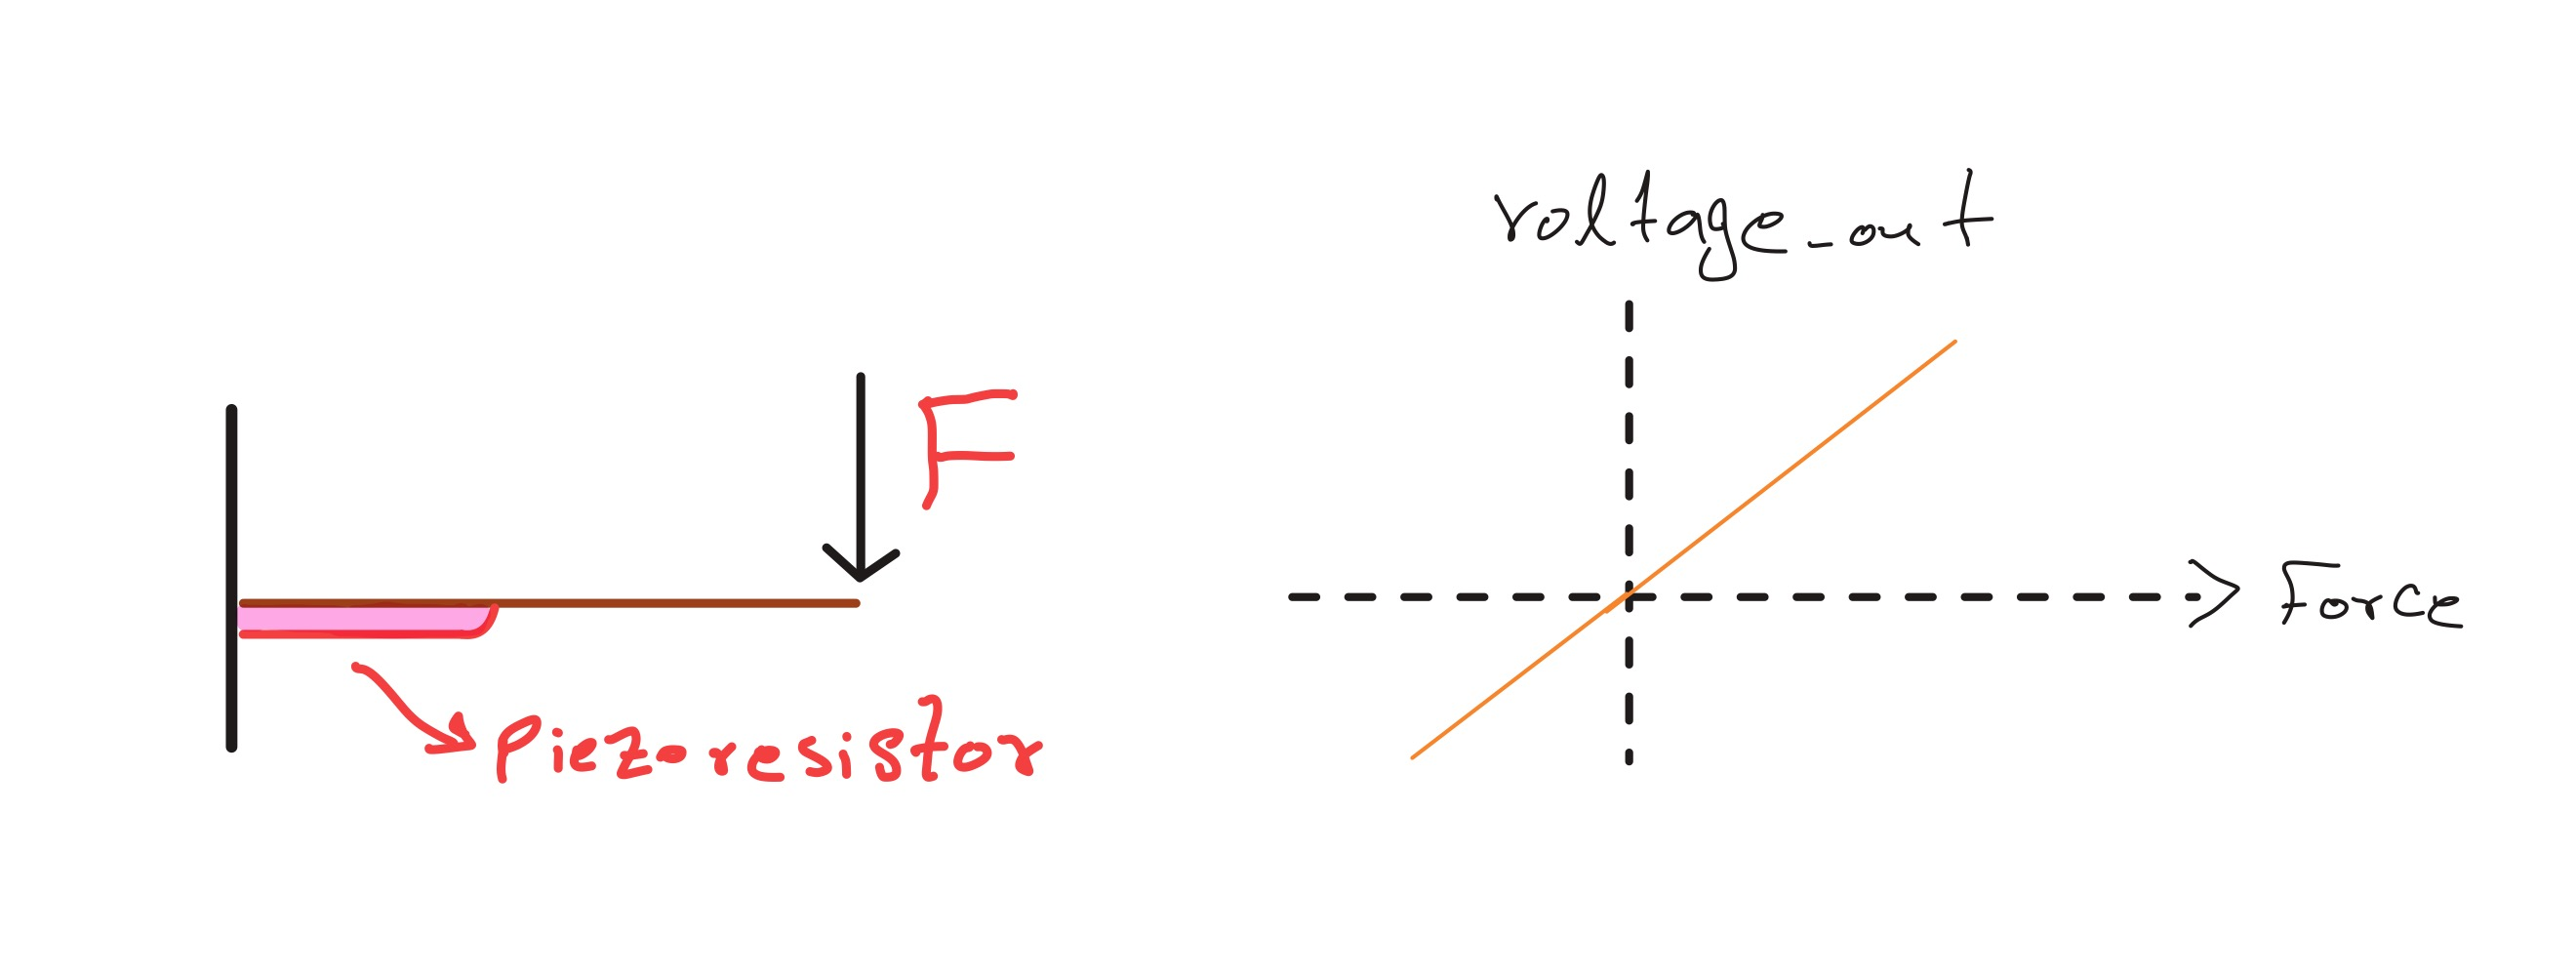
\includegraphics[width=0.5\textwidth]{Images/phenomenon.jpeg}
    \caption{A schematic representation of the piezoresistive effect, where mechanical deformation leads to changes in electrical response.}
\end{figure}

The piezoresistive effect, first observed by William Thomson (Lord Kelvin) 
in the 19th century and later developed for semiconductors by Bardeen, Shockley, and Smith \cite{smith1954}, 
describes the dependence of electrical conductivity on mechanical deformation. 
At a microscopic level, this behavior can be attributed to changes in the electronic structure 
and carrier transport mechanisms induced by strain, which modify quantities such as mobility 
and effective mass.

There exists a wide spectrum of engineering realizations of the piezoresistive effect, 
including strain gauges, pressure sensors, microelectromechanical systems (MEMS), 
cantilever-based sensing devices, and flexible or wearable systems \cite{doll2013}. 
Although these systems differ in geometry, material composition, and boundary conditions, 
they share a common physical origin rooted in the interaction between mechanical deformation 
and electronic transport.

Despite extensive technological development and optimization, the modeling of this coupling 
is often performed in a phenomenological and application-specific manner, where the dependence 
of conductivity on strain is introduced empirically. From a computational materials perspective, 
this raises the question of how such macroscopic descriptions can be related to the underlying 
physical mechanisms governing charge transport.

This work aims to address this by developing a computational framework that captures the 
electromechanical coupling at the continuum level, while maintaining a clear connection to the 
underlying physical processes. In this context, the continuum model serves as an effective 
description of strain-dependent conductivity, providing a bridge between microscopic transport 
phenomena and macroscopic device behavior.